\documentclass{beamer}
\usetheme{Madrid}
\usecolortheme{default}

% Define custom colors for AI slides
\definecolor{AIBlue}{RGB}{30, 144, 255}
\definecolor{AILightBlue}{RGB}{173, 216, 230}
\definecolor{AINavy}{RGB}{25, 25, 112}

% Commands to switch to AI color scheme
\newcommand{\AIcolors}{%
  \setbeamercolor{frametitle}{bg=AIBlue,fg=white}%
  \setbeamercolor{title}{bg=AINavy,fg=white}%
  \setbeamercolor{structure}{fg=AIBlue}%
  \setbeamercolor{item}{fg=AINavy}%
  \setbeamercolor{normal text}{fg=black}%
}

% Command to restore default colors
\newcommand{\defaultcolors}{%
  \setbeamercolor{frametitle}{bg=osaorange,fg=white}%
  \setbeamercolor{title}{bg=osaorange,fg=white}%
  \setbeamercolor{structure}{fg=osaorange}%
  \setbeamercolor{item}{fg=black}%
  \setbeamercolor{normal text}{fg=black}%
}

% Define OSU orange color
\definecolor{osaorange}{RGB}{220,115,38}

% Set colors
\setbeamercolor{structure}{fg=osaorange}
\setbeamercolor{title}{fg=white,bg=osaorange}
\setbeamercolor{frametitle}{fg=white,bg=osaorange}

\usepackage{graphicx}
\usepackage{amsmath}
\usepackage{booktabs}
\usepackage{hyperref}

\title{H524 Introduction to Biostatistics}
\subtitle{Week 1: Introduction to R, Data Presentation, and Summary Measures}
\author{Dr. John Molitor}
\institute{Oregon State University\\College of Health}
\date{Fall 2025}

\begin{document}

\frame{\titlepage}

\begin{frame}
\frametitle{Outline}
\tableofcontents
\end{frame}

\section{Course Introduction}

\begin{frame}
\frametitle{Course Overview}
\begin{itemize}
\item \textbf{Course:} H524 Introduction to Biostatistics
\item \textbf{Credits:} 4 credit hours
\item \textbf{Format:} Online
\item \textbf{Schedule:}
  \begin{itemize}
  \item Lecture: Monday, Wednesday 12:00-1:20pm
  \item Lab: Wednesday 8:00am-9:50am
  \end{itemize}
\item \textbf{Textbook:} Principles of Biostatistics, 2nd edition (Pagano \& Gauvreau)
\end{itemize}
\end{frame}

\begin{frame}
\frametitle{Learning Outcomes}
By the end of this course, you will be able to:
\begin{enumerate}
\item Select and generate graphical and numerical summaries of data
\item Use principles of statistical inference to make conclusions about populations from samples
\item Communicate statistical findings to others
\item Use computer software to conduct statistical analysis
\end{enumerate}
\end{frame}

\begin{frame}
\frametitle{Evaluation}
\begin{center}
\begin{tabular}{lr}
\toprule
\textbf{Component} & \textbf{Weight} \\
\midrule
Homework & 30\% \\
Midterm Exam & 30\% \\
Final Exam & 30\% \\
Class Participation & 10\% \\
\bottomrule
\end{tabular}
\end{center}
\end{frame}

\section{Introduction to R}

\begin{frame}
\frametitle{Why R for Biostatistics?}
\begin{itemize}
\item \textbf{Free and Open Source:} No licensing costs
\item \textbf{Comprehensive:} Extensive statistical capabilities
\item \textbf{Reproducible Research:} Scripts can be saved and shared
\item \textbf{Graphics:} Excellent data visualization capabilities
\item \textbf{Community:} Large user base with extensive documentation
\item \textbf{Packages:} Specialized biostatistics packages available
\end{itemize}
\end{frame}

\begin{frame}
\frametitle{R Basics: Getting Started}
\begin{itemize}
\item \textbf{Console:} Interactive command line
\item \textbf{Scripts:} Save your work in .R files
\item \textbf{Working Directory:} Know where your files are located
\item \textbf{Help System:} Use \texttt{?function\_name} or \texttt{help(function\_name)}
\end{itemize}

\vspace{0.5cm}
Basic commands:
\begin{itemize}
\item \texttt{getwd()} - Check working directory
\item \texttt{setwd()} - Set working directory
\item \texttt{ls()} - List objects in workspace
\item \texttt{rm()} - Remove objects
\end{itemize}
\end{frame}

\begin{frame}[fragile]
\frametitle{R Data Types}
\begin{itemize}
\item \textbf{Numeric:} \texttt{x <- 3.14}
\item \textbf{Integer:} \texttt{y <- 5L}
\item \textbf{Character:} \texttt{name <- "John"}
\item \textbf{Logical:} \texttt{flag <- TRUE}
\item \textbf{Factor:} \texttt{gender <- factor(c("M", "F", "M"))}
\end{itemize}

\vspace{0.5cm}
Data structures:
\begin{itemize}
\item \textbf{Vector:} \texttt{c(1, 2, 3, 4)}
\item \textbf{Matrix:} \texttt{matrix(1:6, nrow=2)}
\item \textbf{Data Frame:} \texttt{data.frame(age=c(25,30), name=c("A","B"))}
\item \textbf{List:} \texttt{list(numbers=1:5, text="hello")}
\end{itemize}
\end{frame}

\section{Data Presentation}

\begin{frame}
\frametitle{Data Sources and Citations}
\textbf{Real datasets from published sources:}

\vspace{0.4cm}
\begin{itemize}
\item \textbf{FEV1 (Lung Function) Data}
  \begin{itemize}
  \item Source: Pagano \& Gauvreau ``Principles of Biostatistics'', pp. 38-39
  \item Study of 13 adolescents with asthma
  \item Variables: FEV1 measurements (liters), gender
  \end{itemize}
\item \textbf{Childhood Injury Deaths}
  \begin{itemize}
  \item Source: Pagano \& Gauvreau ``Principles of Biostatistics'', pp. 24-25
  \item 100 children aged 5-9 who died from injuries, 1980-1985
  \item Variables: Cause of death (categorical)
  \end{itemize}
\end{itemize}

\vspace{0.4cm}
\textbf{Additional sources available:}
\begin{itemize}
\item Serum cholesterol: National Health Examination Survey (pp. 12-15)
\item Birth weight: 3.7 million US births, 1986 (pp. 26-28)
\item All data publicly available through government agencies and published studies
\end{itemize}
\end{frame}

\begin{frame}
\frametitle{Types of Data: Quantitative}
\begin{itemize}
\item \textbf{Quantitative (Numerical Data)}
  \begin{itemize}
  \item \textit{Continuous:} Can take any value within a range
    \begin{itemize}
    \item Blood pressure (120.5 mmHg)
    \item Body temperature (98.6°F)
    \item Cholesterol level (185.3 mg/dL)
    \item Time to recovery (3.5 days)
    \end{itemize}
  \vspace{0.3cm}
  \item \textit{Discrete:} Countable values
    \begin{itemize}
    \item Number of hospitalizations (0, 1, 2, 3...)
    \item Pill count in a bottle (30, 60, 90...)
    \item Number of symptoms reported (1, 2, 3...)
    \item Children in family (0, 1, 2, 3...)
    \end{itemize}
  \end{itemize}
\end{itemize}
\end{frame}

\begin{frame}
\frametitle{Types of Data: Qualitative}
\begin{itemize}
\item \textbf{Qualitative (Categorical Data)}
  \begin{itemize}
  \item \textit{Nominal:} No natural ordering
    \begin{itemize}
    \item Blood type (A, B, AB, O)
    \item Gender (Male, Female, Other)
    \item Insurance type (Private, Medicare, Medicaid)
    \item Medication name (Aspirin, Ibuprofen)
    \end{itemize}
  \vspace{0.3cm}
  \item \textit{Ordinal:} Natural ordering exists
    \begin{itemize}
    \item Pain scale (None, Mild, Moderate, Severe)
    \item Disease stage (Stage I, II, III, IV)
    \item Education level (Less than HS, HS, College, Graduate)
    \item Smoking status (Never, Former, Current)
    \end{itemize}
  \end{itemize}
\end{itemize}
\end{frame}

\begin{frame}
\frametitle{Frequency Distributions}
\textbf{Purpose:} Organize and summarize data

\vspace{0.5cm}
\textbf{For Categorical Data:}
\begin{itemize}
\item Frequency tables
\item Relative frequency (proportions)
\item Percentages
\end{itemize}

\vspace{0.5cm}
\textbf{For Continuous Data:}
\begin{itemize}
\item Group data into intervals (bins)
\item Create frequency tables
\item Choose appropriate number of intervals
\end{itemize}
\end{frame}

\begin{frame}[fragile]
\frametitle{Graphical Displays: Categorical Data}
\begin{itemize}
\item \textbf{Bar Charts}
  \begin{itemize}
  \item Bars separated by spaces
  \item Height represents frequency or percentage
  \item Good for comparing categories
  \end{itemize}
\item \textbf{Pie Charts}
  \begin{itemize}
  \item Shows proportions of a whole
  \item Best for few categories
  \item Less effective for precise comparisons
  \end{itemize}
\end{itemize}

\vspace{0.3cm}
\textbf{R Example:}
\small
\begin{verbatim}
# Create bar chart for education levels
education_counts <- table(survey_data$education)
barplot(education_counts, main = "Education Distribution",
        ylab = "Frequency", col = c("#FF6B35", "#F7931E"))

# Create pie chart for insurance types
insurance_counts <- table(survey_data$insurance)
pie(insurance_counts, main = "Insurance Distribution")
\end{verbatim}
\end{frame}

\begin{frame}
\frametitle{Bar Chart Example}
\begin{center}
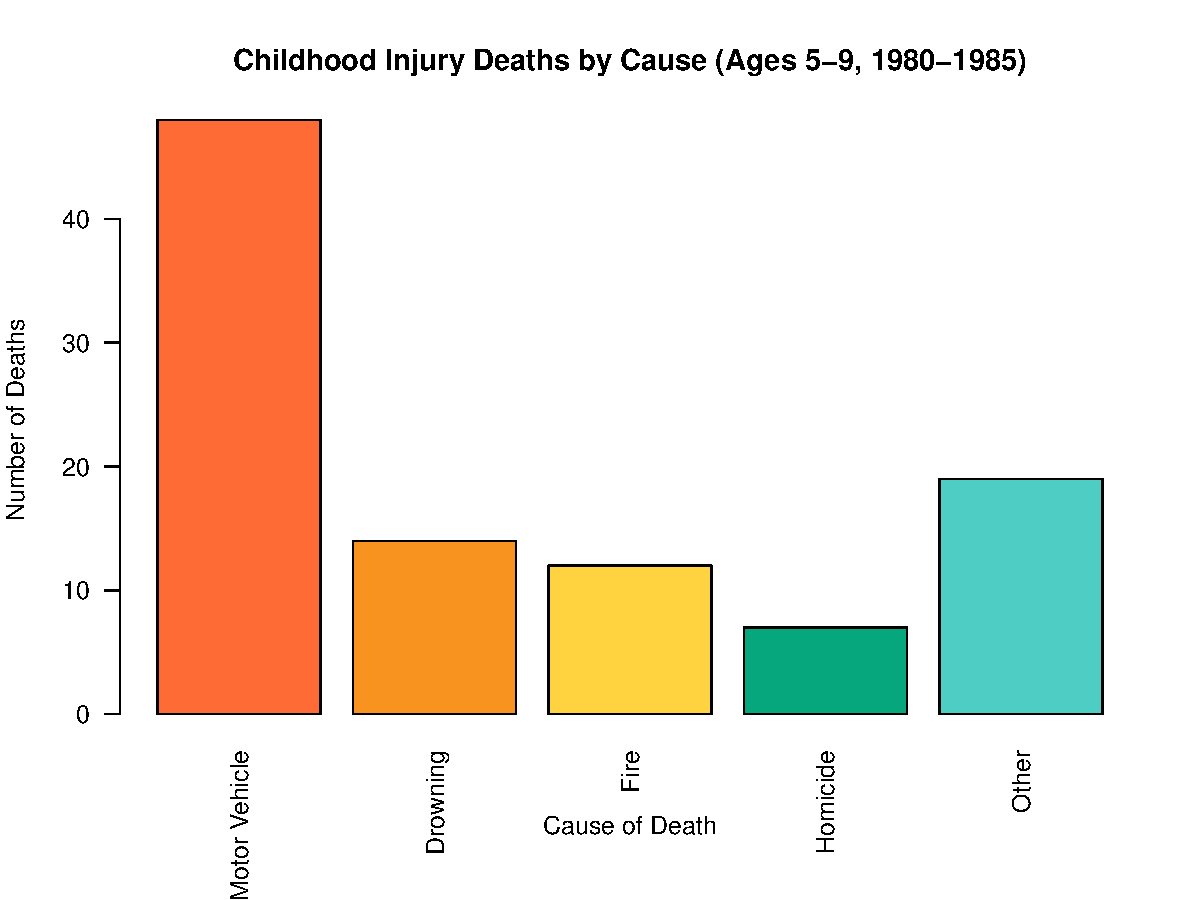
\includegraphics[width=0.8\textwidth, height=0.55\textheight, keepaspectratio]{../code/barplot_injuries.pdf}
\end{center}
\end{frame}

\begin{frame}
\frametitle{Pie Chart Example}
\begin{center}
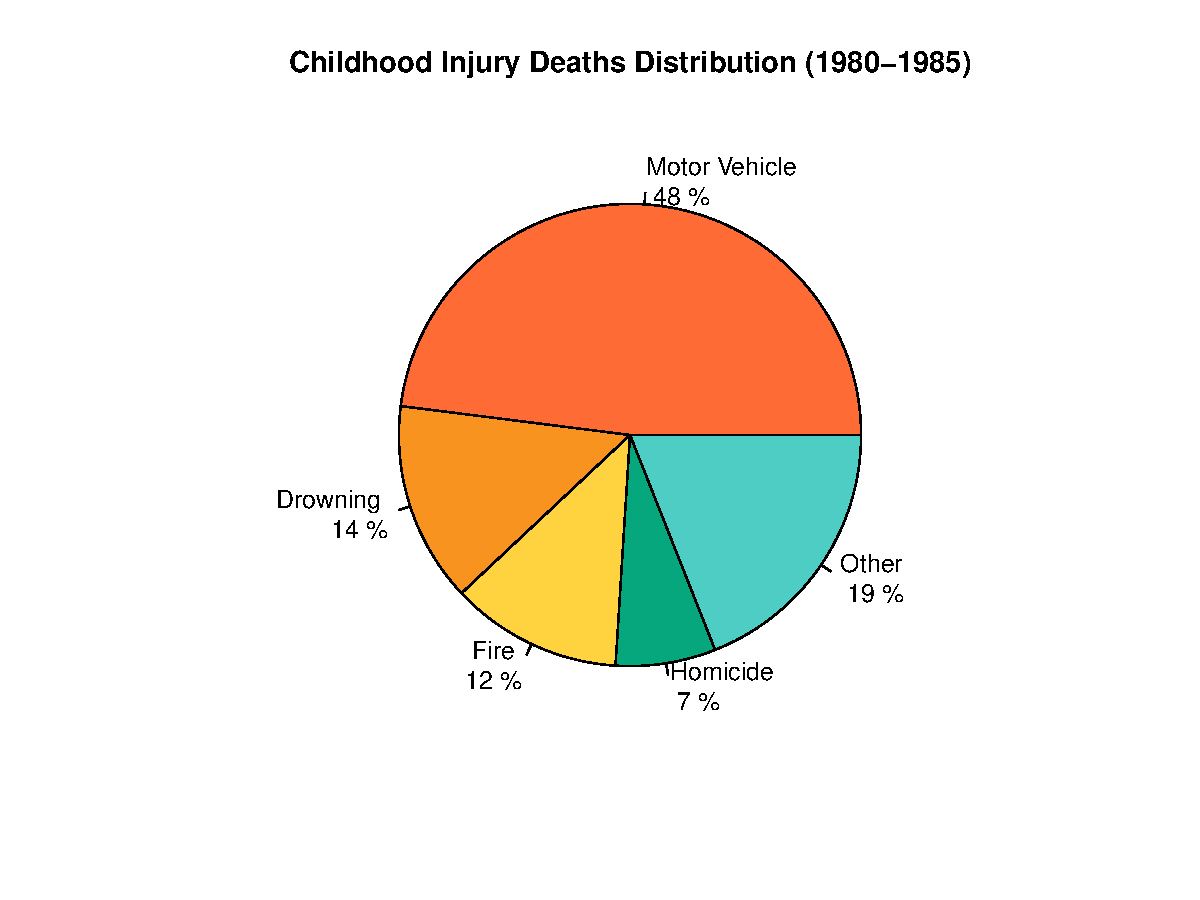
\includegraphics[width=0.8\textwidth, height=0.55\textheight, keepaspectratio]{../code/piechart_injuries.pdf}
\end{center}
\end{frame}

\begin{frame}[fragile]
\frametitle{Graphical Displays: Continuous Data}
\begin{itemize}
\item \textbf{Histograms}
  \begin{itemize}
  \item Bars touch each other
  \item Shows distribution shape
  \item Data is grouped into bins (intervals)
  \item Bin width affects appearance and is somewhat subjective
  \item Different bin choices can reveal different patterns
  \end{itemize}
\item \textbf{Box Plots}
  \begin{itemize}
  \item Shows median, quartiles, outliers
  \item Good for comparing groups
  \item Compact display
  \end{itemize}
\item \textbf{Dot Plots}
  \begin{itemize}
  \item Each observation as a dot
  \item Good for small datasets
  \end{itemize}
\end{itemize}

\vspace{0.2cm}
\textbf{R Example:}
\tiny
\begin{verbatim}
# Histogram for BMI distribution
hist(health_data$bmi, main = "BMI Distribution",
     xlab = "BMI", col = "#FF6B35")

# Box plot for blood pressure
boxplot(health_data$systolic_bp, main = "BP Distribution")
\end{verbatim}
\end{frame}

\begin{frame}
\frametitle{Histogram Example}
\begin{center}
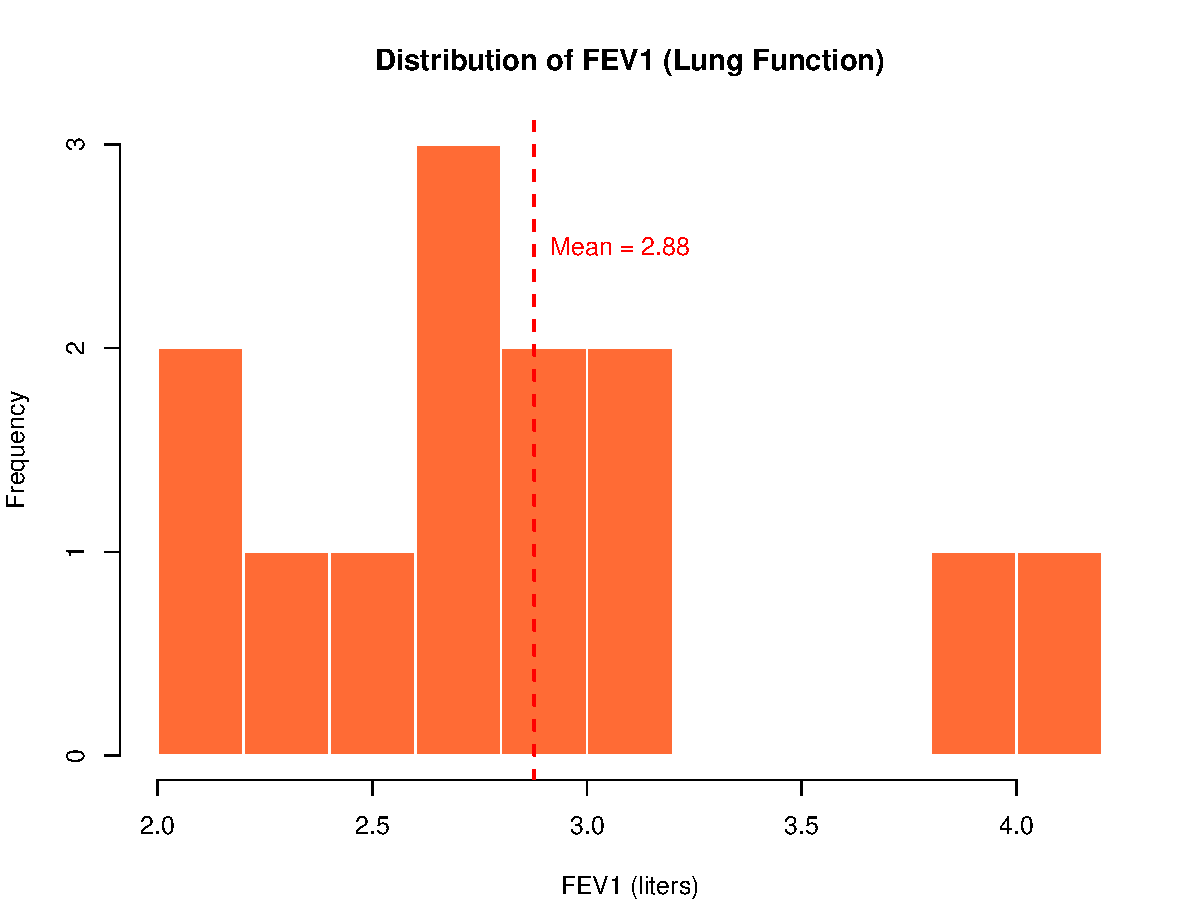
\includegraphics[width=0.8\textwidth, height=0.55\textheight, keepaspectratio]{../code/histogram_fev1.pdf}
\end{center}
\end{frame}

\begin{frame}
\frametitle{Box Plot Example}
\begin{center}
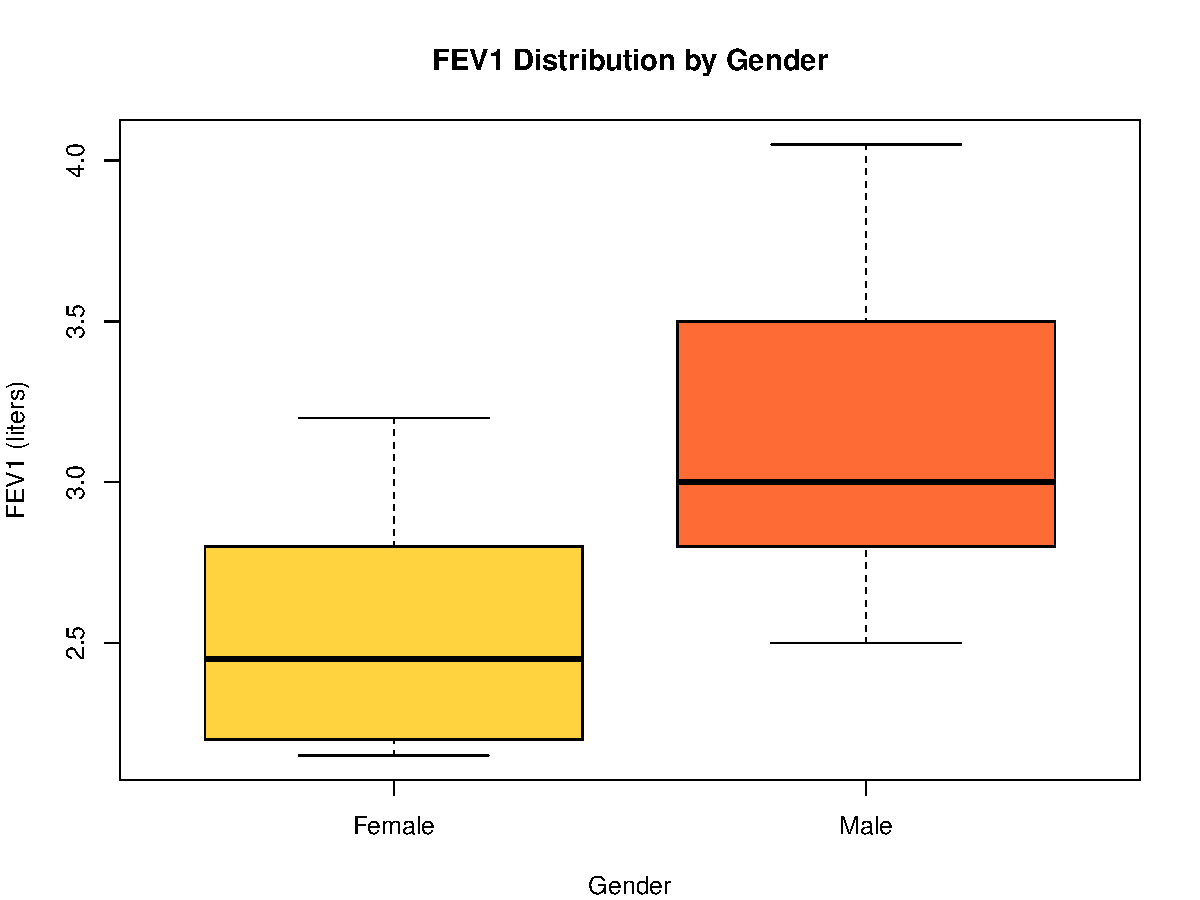
\includegraphics[width=0.8\textwidth, height=0.55\textheight, keepaspectratio]{../code/boxplot_fev1_gender.pdf}
\end{center}
\end{frame}

\begin{frame}
\frametitle{Dot Plot Example}
\begin{center}
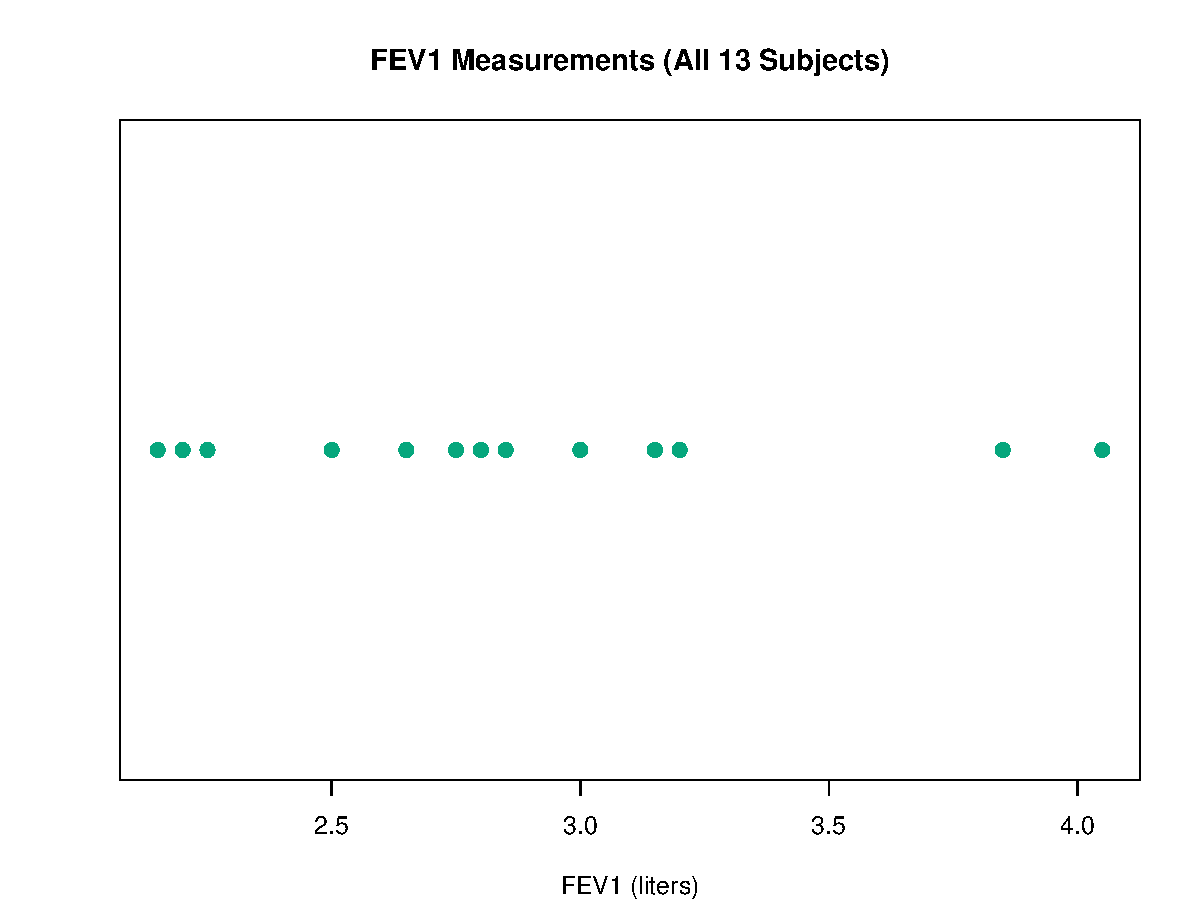
\includegraphics[width=0.8\textwidth, height=0.55\textheight, keepaspectratio]{../code/dotplot_fev1.pdf}
\end{center}
\end{frame}

\begin{frame}
\frametitle{Scatter Plot Example}
\begin{center}
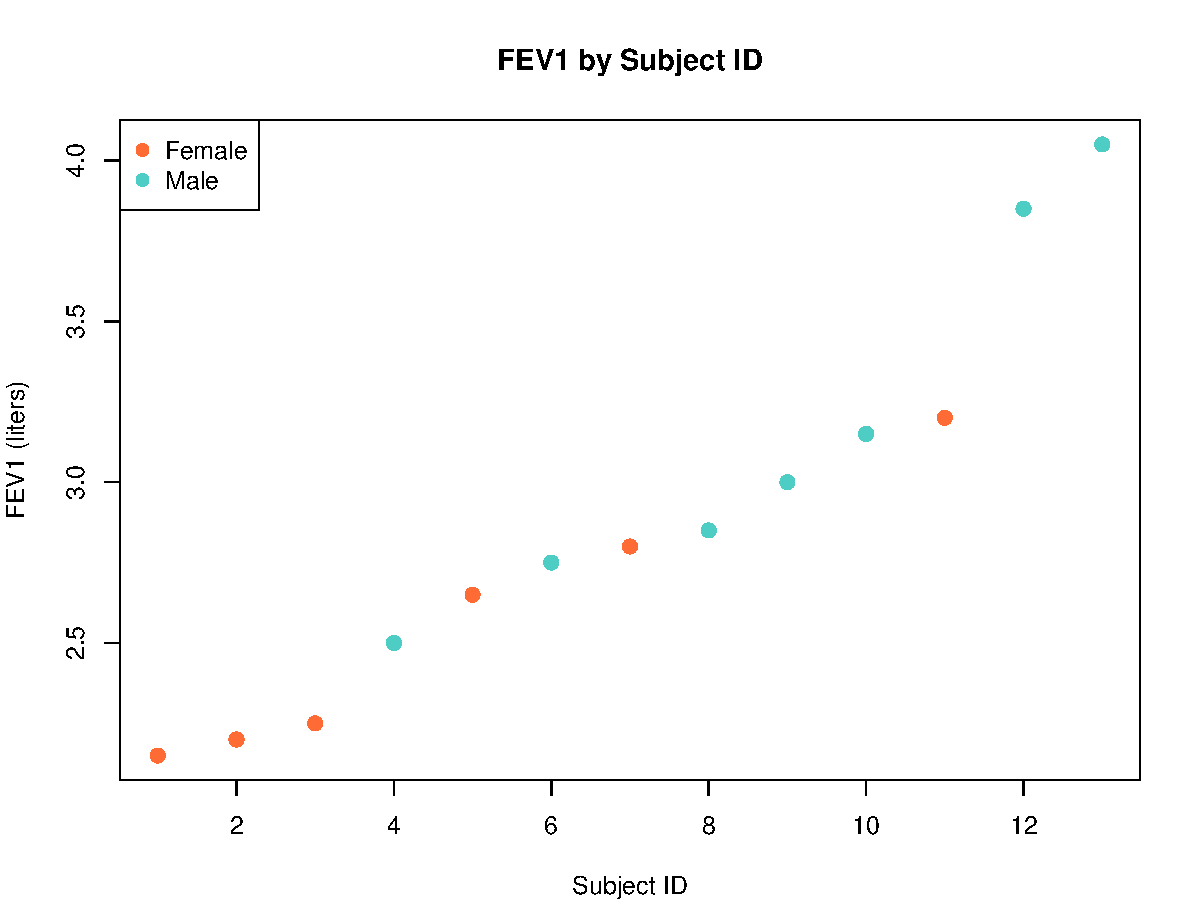
\includegraphics[width=0.8\textwidth, height=0.55\textheight, keepaspectratio]{../code/scatter_fev1.pdf}
\end{center}
\end{frame}

\section{Numerical Summary Measures}

\begin{frame}
\frametitle{Measures of Central Tendency}
\begin{itemize}
\item \textbf{Mean ($\bar{x}$)}
  \begin{itemize}
  \item $\bar{x} = \frac{\sum_{i=1}^{n} x_i}{n}$
  \item Sensitive to outliers
  \item Most common measure
  \end{itemize}
\item \textbf{Median}
  \begin{itemize}
  \item Middle value when data is ordered
  \item Resistant to outliers
  \item Good for skewed distributions
  \end{itemize}
\item \textbf{Mode}
  \begin{itemize}
  \item Most frequently occurring value
  \item Can have multiple modes
  \item Useful for categorical data
  \end{itemize}
\end{itemize}
\end{frame}

\begin{frame}
\frametitle{Measures of Variability}
\begin{itemize}
\item \textbf{Range}
  \begin{itemize}
  \item Maximum - Minimum
  \item Simple but sensitive to outliers
  \end{itemize}
\item \textbf{Variance ($s^2$)}
  \begin{itemize}
  \item $s^2 = \frac{\sum_{i=1}^{n} (x_i - \bar{x})^2}{n-1}$
  \item Average squared deviation from mean
  \end{itemize}
\item \textbf{Standard Deviation ($s$)}
  \begin{itemize}
  \item $s = \sqrt{s^2}$
  \item Same units as original data
  \end{itemize}
\end{itemize}
\end{frame}

\begin{frame}
\frametitle{Percentiles and Quartiles}
\begin{itemize}
\item \textbf{Percentiles:} Value below which a certain percentage of data falls
\item \textbf{Quartiles:} Divide data into four equal parts
  \begin{itemize}
  \item Q1 (25th percentile): First quartile
  \item Q2 (50th percentile): Median
  \item Q3 (75th percentile): Third quartile
  \end{itemize}
\item \textbf{Interquartile Range (IQR):} Q3 - Q1
  \begin{itemize}
  \item Contains middle 50\% of data
  \item Resistant to outliers
  \end{itemize}
\end{itemize}
\end{frame}

\section{Rates and Standardization}

\begin{frame}
\frametitle{Introduction to Rates}
\textbf{Rate:} A measure of the frequency of occurrence of an event

\vspace{0.5cm}
General form:
$$\text{Rate} = \frac{\text{Number of events}}{\text{Population at risk}} \times k$$

where $k$ is a constant (often 1,000, 10,000, or 100,000)

\vspace{0.5cm}
\textbf{Why use rates?}
\begin{itemize}
\item Enable comparison between populations of different sizes
\item Standardize measurements across time periods
\item Account for population at risk
\end{itemize}
\end{frame}

\begin{frame}
\frametitle{Common Types of Rates}
\begin{itemize}
\item \textbf{Crude Birth Rate}
  $$\frac{\text{Number of births in a year}}{\text{Total population}} \times 1000$$

\item \textbf{Crude Death Rate}
  $$\frac{\text{Number of deaths in a year}}{\text{Total population}} \times 1000$$

\item \textbf{Disease Incidence Rate}
  $$\frac{\text{New cases of disease}}{\text{Population at risk}} \times k$$

\item \textbf{Case Fatality Rate}
  $$\frac{\text{Deaths from disease}}{\text{Total cases of disease}} \times 100$$
\end{itemize}
\end{frame}

\begin{frame}
\frametitle{Age-Specific Rates}
\textbf{Problem:} Crude rates can be misleading when comparing populations with different age structures

\vspace{0.5cm}
\textbf{Solution:} Calculate rates for specific age groups

$$\text{Age-specific rate} = \frac{\text{Events in age group}}{\text{Population in age group}} \times k$$

\vspace{0.5cm}
\textbf{Advantages:}
\begin{itemize}
\item More precise comparisons
\item Accounts for age distribution differences
\item Reveals age-related patterns
\end{itemize}
\end{frame}

\begin{frame}
\frametitle{Age Standardization}
\textbf{Direct Method:}
\begin{enumerate}
\item Apply age-specific rates from each population to a standard population
\item Sum across age groups
\item Compare standardized rates
\end{enumerate}

\vspace{0.5cm}
$$\text{Directly standardized rate} = \frac{\sum_{i} R_i \times P_{i}^{std}}{\sum_{i} P_{i}^{std}} \times k$$

where:
\begin{itemize}
\item $R_i$ = age-specific rate for age group $i$
\item $P_{i}^{std}$ = standard population size for age group $i$
\end{itemize}
\end{frame}

\begin{frame}
\frametitle{Age Standardization (continued)}
\textbf{Indirect Method:}
\begin{enumerate}
\item Apply standard age-specific rates to study population
\item Calculate expected number of events
\item Compare observed vs. expected
\end{enumerate}

\vspace{0.5cm}
$$\text{SMR} = \frac{\text{Observed events}}{\text{Expected events}} \times 100$$

\textbf{SMR} = Standardized Mortality Ratio
\begin{itemize}
\item SMR $>$ 100: Higher than expected
\item SMR $<$ 100: Lower than expected
\item SMR $=$ 100: Same as expected
\end{itemize}
\end{frame}

\section{AI as a Learning Tool}

\AIcolors
\begin{frame}
\frametitle{AI in Biostatistics: A Modern Learning Tool}
\begin{itemize}
\item \textbf{AI tools can enhance learning} but cannot replace understanding
\item \textbf{Use AI as a statistical tutor} that requires supervision
\item \textbf{Critical evaluation} of AI output is essential
\item \textbf{Maintain statistical rigor} while leveraging AI assistance
\end{itemize}

\vspace{0.5cm}
\textbf{Today's Goal:} Learn to use AI effectively for biostatistics

\vspace{0.5cm}
\textbf{Popular AI Tools:}
\begin{itemize}
\item ChatGPT, Claude (used in today's demos), Copilot
\item R-specific: GitHub Copilot for R
\item Statistical help: Wolfram Alpha
\end{itemize}
\end{frame}

\begin{frame}[fragile]
\frametitle{AI Demo 1: Generating R Code}
\textbf{Prompt:} ``Create R code to calculate descriptive statistics for blood pressure data''

\vspace{0.3cm}
\textbf{Claude AI Response:}
\tiny
\begin{verbatim}
# First, load the real data from our Week 1 script
source("week1_lecture_code.R")
# This creates fev1_data with FEV1 measurements from real study

# Calculate descriptive statistics for FEV1 data
mean_fev1 <- mean(fev1_data$fev1_liters, na.rm = TRUE)
median_fev1 <- median(fev1_data$fev1_liters, na.rm = TRUE)
sd_fev1 <- sd(fev1_data$fev1_liters, na.rm = TRUE)
min_fev1 <- min(fev1_data$fev1_liters, na.rm = TRUE)
max_fev1 <- max(fev1_data$fev1_liters, na.rm = TRUE)

# Display results
cat("Mean FEV1:", round(mean_fev1, 2), "liters\n")
cat("Median FEV1:", round(median_fev1, 2), "liters\n")
cat("SD:", round(sd_fev1, 2), "liters\n")
cat("Range:", min_fev1, "-", max_fev1, "liters\n")

# Alternative: use summary function
summary(fev1_data$fev1_liters)
\end{verbatim}

\vspace{0.2cm}
\textbf{What to check:} Variable names, missing value handling, appropriate functions
\end{frame}

\begin{frame}[fragile]
\frametitle{AI Demo 2: Creating Visualizations}
\textbf{Prompt:} ``Create a professional histogram of blood pressure data with normal curve overlay''

\vspace{0.3cm}
\textbf{Claude AI Response:}
\tiny
\begin{verbatim}
# Assumes bp_data is already loaded (from week1_lecture_code.R)
# Create histogram with normal curve overlay
hist(bp_data$systolic_bp,
     breaks = 15,
     probability = TRUE,  # Use density instead of frequency
     main = "Distribution of Systolic Blood Pressure",
     xlab = "Systolic BP (mmHg)",
     ylab = "Density",
     col = "lightblue",
     border = "white")

# Add normal curve overlay
x_vals <- seq(min(bp_data$systolic_bp), max(bp_data$systolic_bp), length = 100)
mean_val <- mean(bp_data$systolic_bp)
sd_val <- sd(bp_data$systolic_bp)
y_vals <- dnorm(x_vals, mean = mean_val, sd = sd_val)
lines(x_vals, y_vals, col = "red", lwd = 2)

# Add vertical line for mean
abline(v = mean_val, col = "darkred", lwd = 2, lty = 2)
legend("topright", c("Normal Curve", "Mean"),
       col = c("red", "darkred"), lwd = 2, lty = c(1, 2))
\end{verbatim}
\end{frame}

\begin{frame}
\frametitle{AI Demo 3: Explaining Statistical Concepts}
\textbf{Student Question:} ``When should I use median instead of mean for blood pressure data?''

\vspace{0.3cm}
\textbf{Claude AI Response:}
\begin{itemize}
\item \textbf{Use median when:}
  \begin{itemize}
  \item Data has outliers (very high/low BP readings)
  \item Distribution is skewed (not bell-shaped)
  \item Want robust measure unaffected by extreme values
  \end{itemize}
\item \textbf{Use mean when:}
  \begin{itemize}
  \item Data is approximately normally distributed
  \item No significant outliers present
  \item Need measure that uses all data points
  \end{itemize}
\item \textbf{For blood pressure:} Often use median because BP can have extreme values due to measurement errors or acute conditions
\end{itemize}

\vspace{0.3cm}
\textbf{Always verify:} Check your actual data distribution before deciding!
\end{frame}

\begin{frame}[fragile]
\frametitle{AI Demo 4: Interpreting Results}
\textbf{Prompt:} ``Interpret these blood pressure analysis results for a health class''

\tiny
\begin{verbatim}
Summary Statistics:
Mean: 133.6 mmHg, SD: 18.6 mmHg
Median: 131.0 mmHg, Range: 96-196 mmHg
Males: Mean = 136.2 mmHg, Females: Mean = 130.8 mmHg
\end{verbatim}

\normalsize
\textbf{Claude AI Interpretation:}
\begin{itemize}
\item \textbf{Central tendency:} Average BP (133.6) is in "high normal" range (AHA guidelines: <120 normal, 120-129 elevated, 130+ high)
\item \textbf{Variability:} Large SD (18.6) indicates substantial individual differences
\item \textbf{Distribution:} Mean > median suggests slight right skew (some high outliers)
\item \textbf{Gender difference:} Males average 5.4 mmHg higher (typical pattern)
\item \textbf{Range:} Wide range (96-196) includes both hypotensive and severely hypertensive readings
\end{itemize}

\textbf{Clinical relevance:} About 30\% of this population likely has hypertension requiring medical attention
\end{frame}

\begin{frame}
\frametitle{AI Best Practices for Biostatistics}
\small
\begin{columns}
\begin{column}{0.5\textwidth}
\textbf{DO:}
\begin{itemize}
\item Start with specific, clear prompts
\item Ask for explanations of code
\item Request multiple approaches
\item Verify results independently
\item Ask for biological context
\item Use AI to check your work
\end{itemize}
\end{column}

\begin{column}{0.5\textwidth}
\textbf{DON'T:}
\begin{itemize}
\item Blindly copy-paste code
\item Skip understanding the logic
\item Use without domain knowledge
\item Ignore warning messages
\item Accept first response
\item Replace critical thinking
\end{itemize}
\end{column}
\end{columns}

\vspace{0.2cm}
\textbf{Golden Rule:} AI should enhance your learning, not replace it
\end{frame}

\begin{frame}
\frametitle{Common AI Pitfalls in Statistics}
\small
\begin{itemize}
\item \textbf{Outdated Information:} AI training data may not include latest statistical methods
\item \textbf{Context Confusion:} May suggest inappropriate tests for biomedical data
\item \textbf{Assumption Violations:} Doesn't always check statistical assumptions
\item \textbf{Missing Values:} May not handle missing data appropriately
\item \textbf{Interpretation Errors:} Can confuse correlation with causation
\item \textbf{Package Dependencies:} May suggest functions from packages you don't have
\end{itemize}

\vspace{0.1cm}
\textbf{Always:}
\begin{itemize}
\item Check your data fits the suggested method
\item Verify assumptions are met
\item Cross-reference with textbooks/course materials
\item Test code on small examples first
\end{itemize}
\end{frame}

\begin{frame}[fragile]
\frametitle{Effective Prompting for Biostatistics}
\textbf{Poor Prompt:}
\texttt{``Help with statistics''}

\vspace{0.3cm}
\textbf{Better Prompt:}
\texttt{``I have blood pressure data from 100 patients. Create R code to compare BP between males and females using appropriate statistical test.''}

\vspace{0.3cm}
\textbf{Best Prompt:}
\small
\begin{verbatim}
``I have blood pressure data from 100 patients with variables:
age, gender, systolic_bp, treatment_group. I want to:
1. Compare systolic BP between males and females
2. Check if data meets normality assumptions
3. Choose appropriate statistical test
4. Interpret results in clinical context
5. Create publication-quality plot
Please provide R code with explanations.''
\end{verbatim}

\normalsize
\textbf{Key elements:} Context, sample size, variables, specific goals, level of explanation needed
\end{frame}

\begin{frame}
\frametitle{AI Assignment Preview}
\textbf{This week's homework will include:}
\begin{enumerate}
\item Using AI to generate R code for data analysis
\item Comparing AI output with manual coding
\item Identifying and correcting AI errors
\item Writing effective statistical prompts
\item Critical evaluation of AI explanations
\end{enumerate}

\vspace{0.5cm}
\textbf{Learning Goals:}
\begin{itemize}
\item Develop AI literacy for biostatistics
\item Maintain statistical rigor while using AI tools
\item Build confidence in statistical computing
\item Prepare for modern data science workflows
\end{itemize}

\vspace{0.5cm}
\textbf{Remember:} AI is a powerful tool, but you are the biostatistician!
\end{frame}

\defaultcolors

\section{R Examples}

\begin{frame}[fragile]
\frametitle{R Example: Blood Pressure Study Data}
\small
\begin{verbatim}
# To follow along: source the complete script
source("week1_lecture_code.R")

# Or generate the data yourself:
set.seed(123)
bp_data <- data.frame(
  age = round(rnorm(100, mean = 45, sd = 15)),
  gender = sample(c("Male", "Female"), 100, replace = TRUE),
  systolic_bp = round(rnorm(100, mean = 130, sd = 20)),
  treatment = sample(c("Control", "Treatment A", "Treatment B"),
                    100, replace = TRUE)
)

# Basic descriptive statistics
mean(bp_data$systolic_bp)     # Mean: 133.6 mmHg
sd(bp_data$systolic_bp)       # SD: 18.6 mmHg
summary(bp_data$systolic_bp)  # Five-number summary
\end{verbatim}
\end{frame}

\begin{frame}
\frametitle{Data Visualization: Histogram}
\vspace{-0.2cm}
\begin{center}
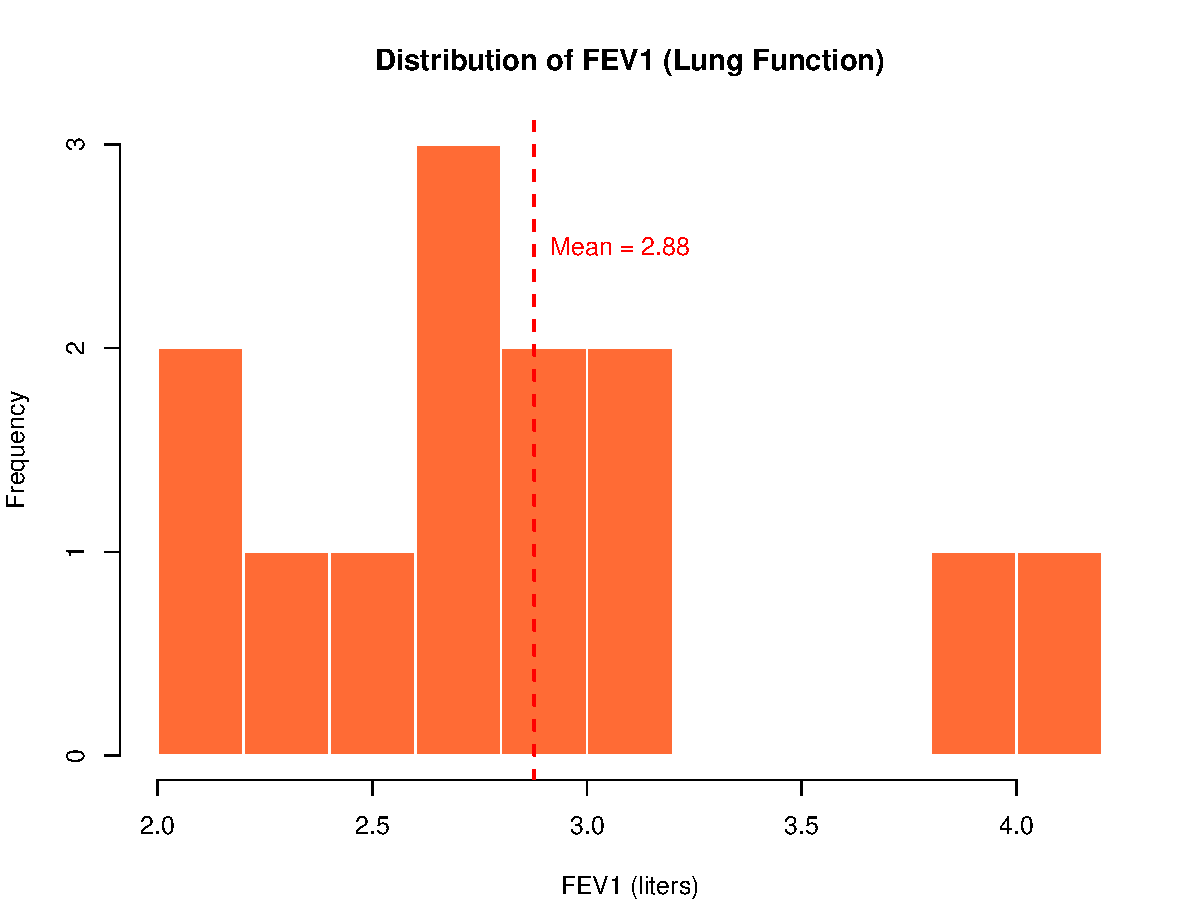
\includegraphics[width=0.8\textwidth, height=0.55\textheight, keepaspectratio]{../code/histogram_fev1.pdf}
\end{center}
\vspace{-0.1cm}
\begin{itemize}
\item Shows distribution of FEV1 lung function measurements
\item Red dashed line indicates mean value (2.88 liters)
\item Real data from 13 adolescents with asthma
\end{itemize}
\end{frame}

\begin{frame}
\frametitle{Data Visualization: Box Plots}
\vspace{-0.2cm}
\begin{center}
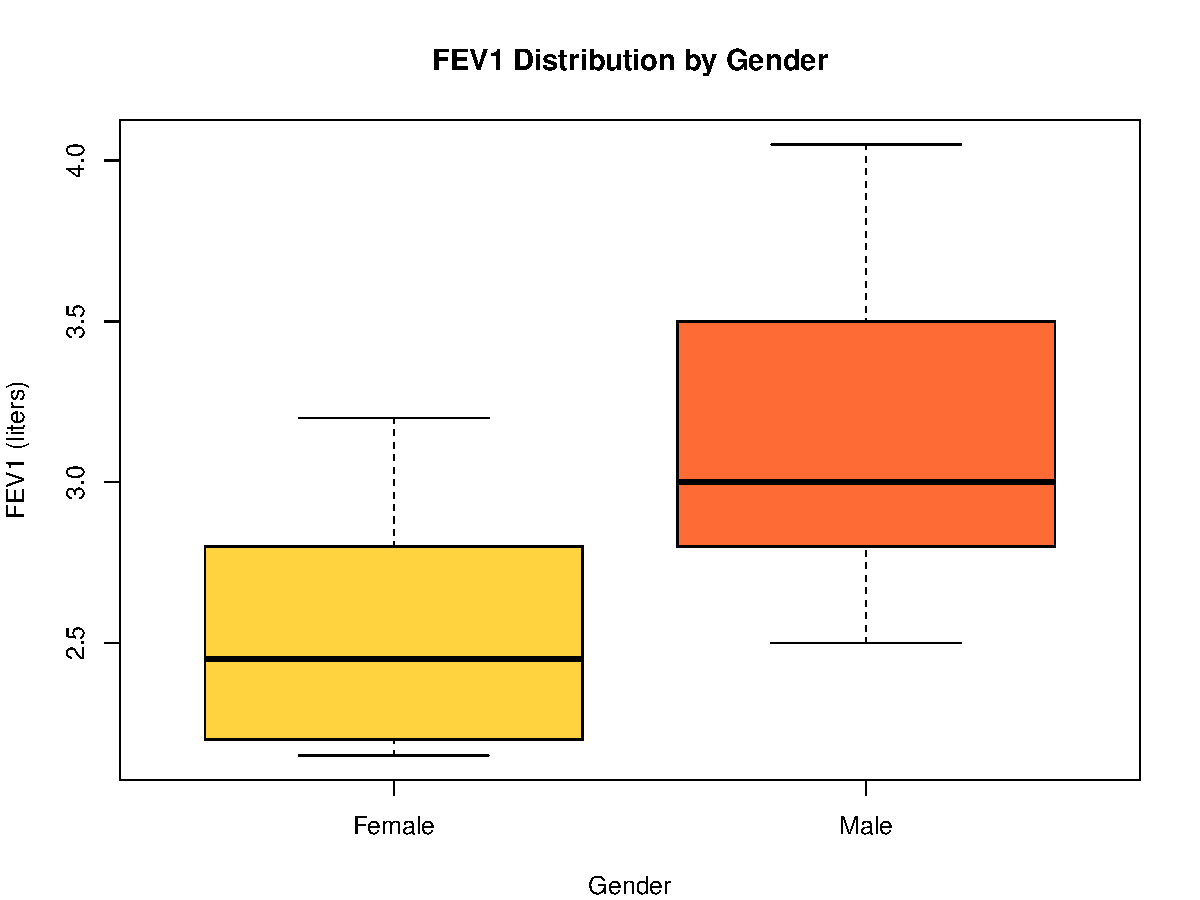
\includegraphics[width=0.8\textwidth, height=0.55\textheight, keepaspectratio]{../code/boxplot_fev1_gender.pdf}
\end{center}
\vspace{-0.1cm}
\begin{itemize}
\item Compares FEV1 distributions between genders
\item Shows median, quartiles, and outliers
\item Males have higher median FEV1 than females
\end{itemize}
\end{frame}

\begin{frame}
\frametitle{Data Visualization: Bar Charts}
\vspace{-0.2cm}
\begin{center}
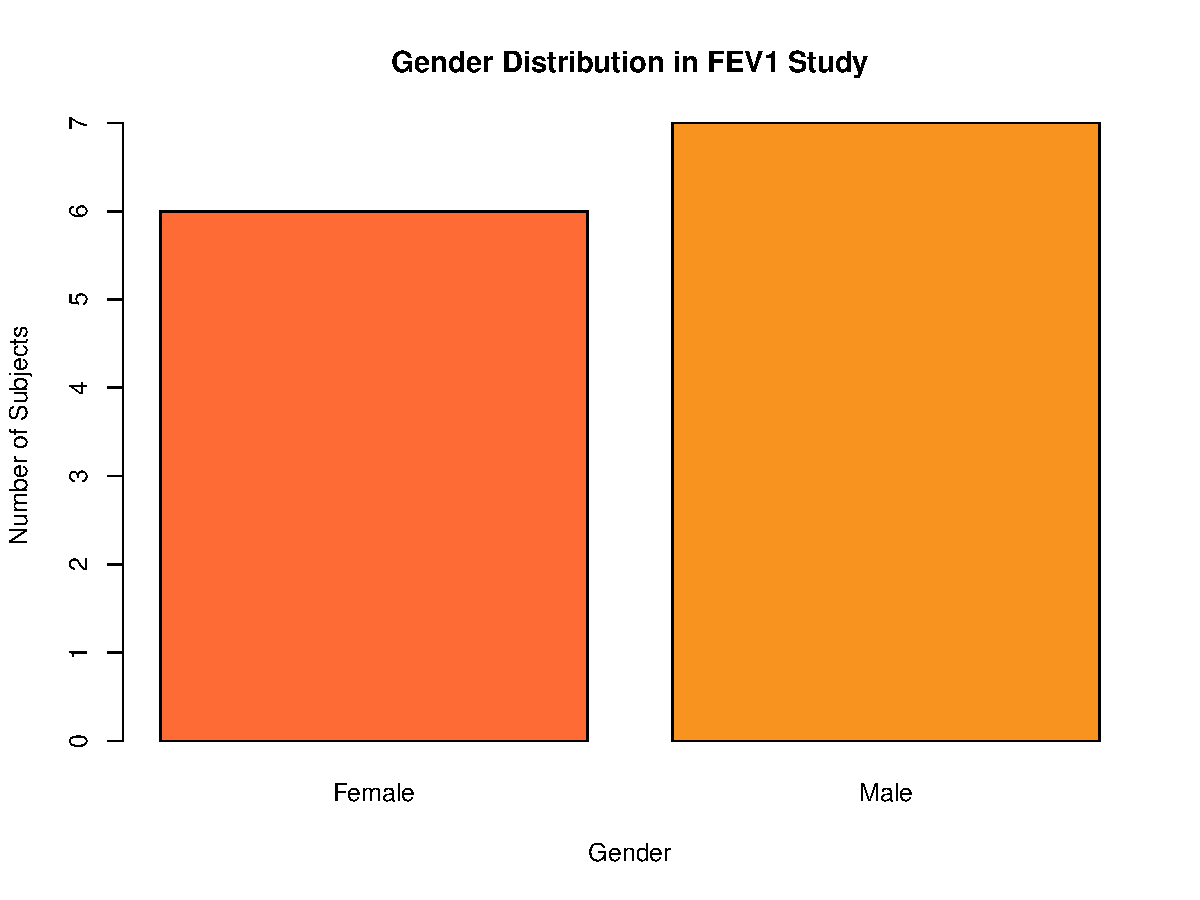
\includegraphics[width=0.8\textwidth, height=0.55\textheight, keepaspectratio]{../code/barplot_gender_fev1.pdf}
\end{center}
\vspace{-0.1cm}
\begin{itemize}
\item Good for categorical data
\item Shows frequency counts for gender in FEV1 study
\item 6 females, 7 males in the study
\end{itemize}
\end{frame}

\begin{frame}
\frametitle{Data Visualization: Scatter Plots}
\vspace{-0.2cm}
\begin{center}
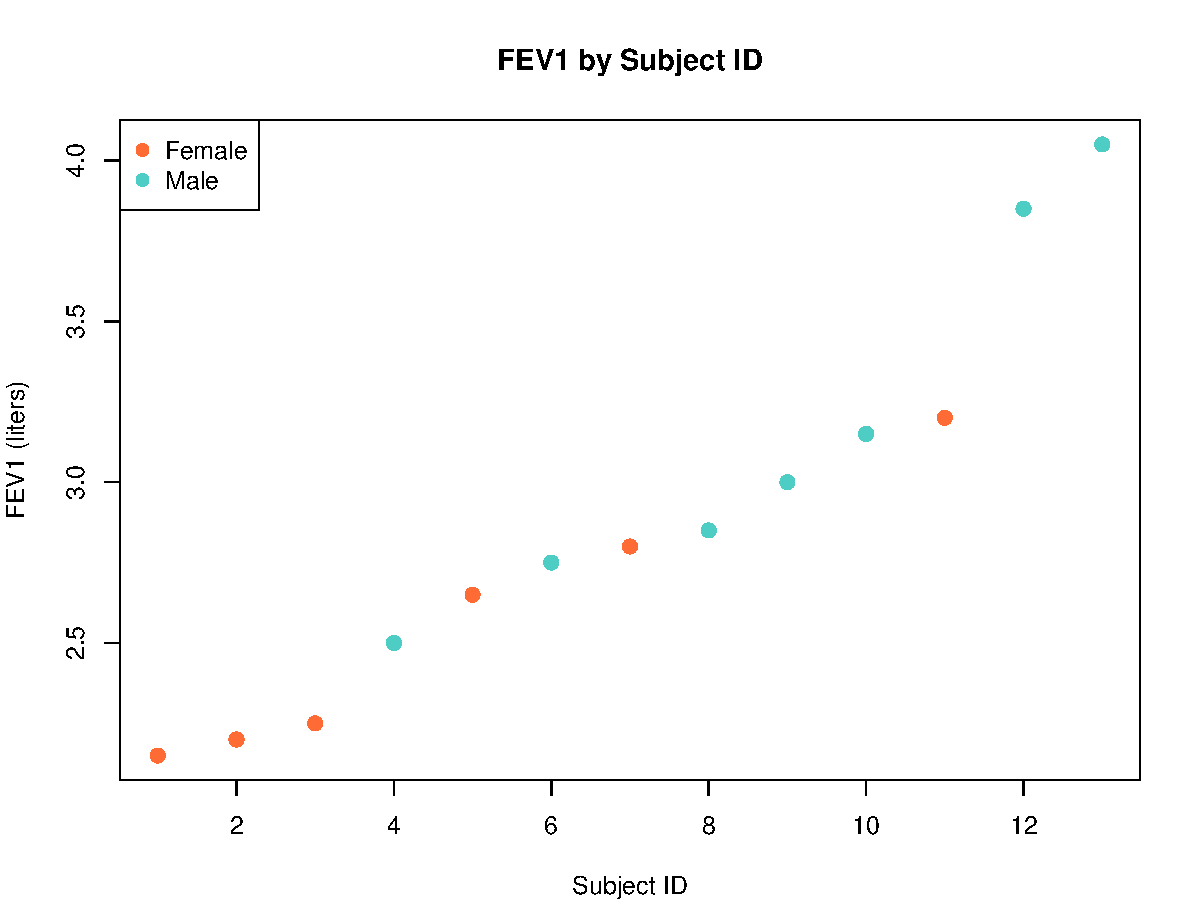
\includegraphics[width=0.8\textwidth, height=0.55\textheight, keepaspectratio]{../code/scatter_fev1.pdf}
\end{center}
\vspace{-0.1cm}
\begin{itemize}
\item Shows FEV1 by subject ID, colored by gender
\item No clear pattern with subject ID
\item Illustrates gender differences in lung function
\end{itemize}
\end{frame}

\begin{frame}[fragile]
\frametitle{R Code: Creating Visualizations}
\tiny
\begin{verbatim}
# Histogram
hist(bp_data$systolic_bp,
     main = "Distribution of Systolic Blood Pressure",
     xlab = "Systolic BP (mmHg)", col = "lightblue")

# Box plot by gender
boxplot(systolic_bp ~ gender, data = bp_data,
        main = "Systolic Blood Pressure by Gender",
        col = c("pink", "lightblue"))

# Scatter plot with regression line
plot(bp_data$age, bp_data$systolic_bp,
     xlab = "Age (years)", ylab = "Systolic BP (mmHg)")
abline(lm(systolic_bp ~ age, data = bp_data), col = "red")
\end{verbatim}
\end{frame}

\begin{frame}[fragile]
\frametitle{R Example: Rates Calculation}
\small
\begin{verbatim}
# Disease surveillance data
population_size <- 50000
new_cases <- 125
deaths <- 15

# Calculate incidence rate
incidence_rate <- (new_cases / population_size) * 100000
# Result: 250 per 100,000 population

# Calculate case fatality rate
case_fatality_rate <- (deaths / new_cases) * 100
# Result: 12%

# Age-specific rates
population_by_age <- c(12000, 15000, 18000, 5000)
cases_by_age <- c(5, 25, 65, 30)
age_specific_rates <- (cases_by_age / population_by_age) * 100000
\end{verbatim}
\end{frame}

\begin{frame}
\frametitle{Age-Specific Rates Visualization}
\vspace{-0.2cm}
\begin{center}
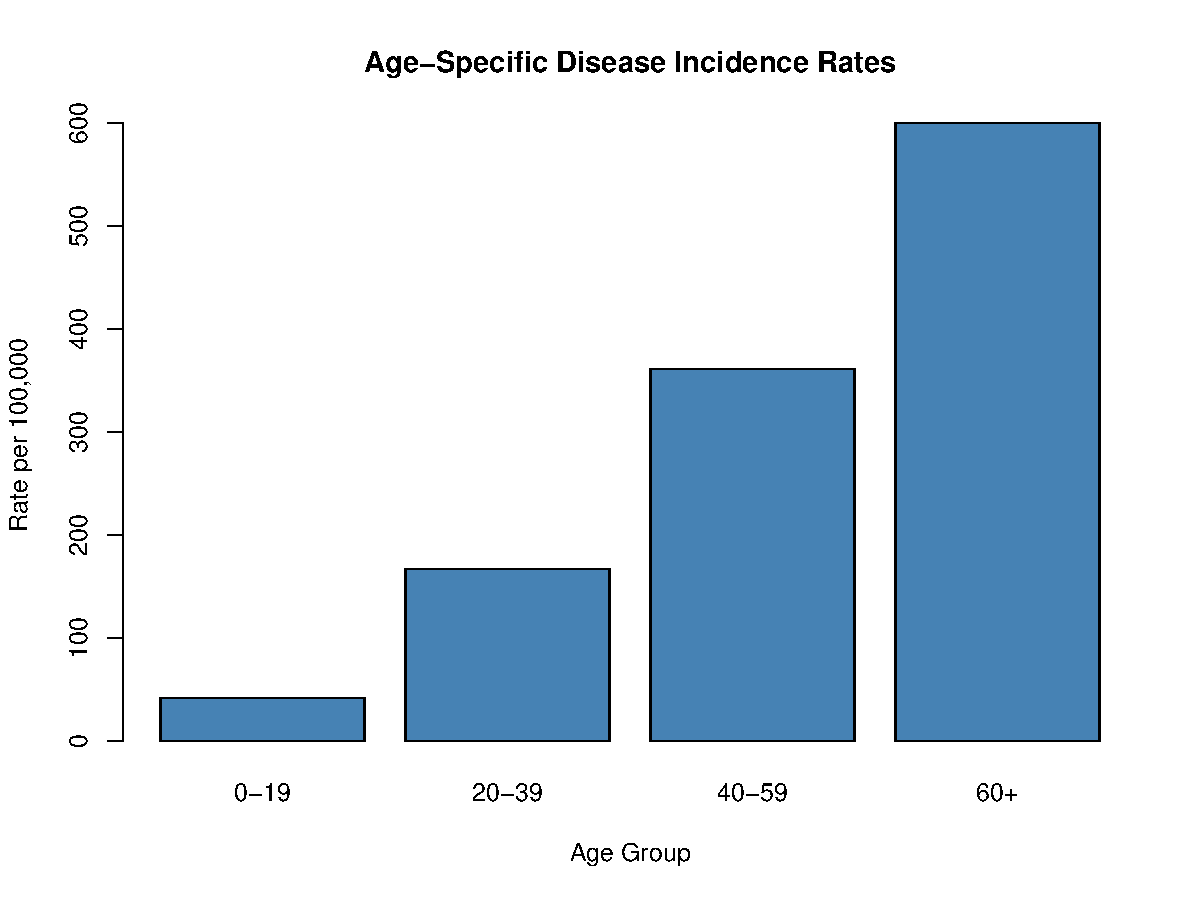
\includegraphics[width=0.8\textwidth, height=0.55\textheight, keepaspectratio]{../code/age_specific_rates.pdf}
\end{center}
\vspace{-0.1cm}
\begin{itemize}
\item Clear age gradient in disease incidence
\item Highest rates in oldest age group (600 per 100,000)
\item Demonstrates importance of age-specific analysis
\end{itemize}
\end{frame}

\begin{frame}
\frametitle{Summary}
\textbf{Today we covered:}
\begin{itemize}
\item Introduction to R and its capabilities
\item Types of data and appropriate presentation methods
\item Graphical displays for different data types
\item Numerical summary measures (central tendency and variability)
\item Rates and age standardization methods
\end{itemize}

\vspace{0.5cm}
\textbf{Next week:} We'll dive deeper into probability concepts

\vspace{0.5cm}
\textbf{Reading:} Pagano \& Gauvreau, Chapters 1-4
\end{frame}

\begin{frame}
\frametitle{Questions?}
\begin{center}
\Large{Thank you!}

\vspace{1cm}

\textbf{Office Hours:} Wednesday, 10:00 am -- 11:30 am\\
\textbf{Email:} john.molitor@oregonstate.edu\\
\textbf{Office:} 153 Milam
\end{center}
\end{frame}

\end{document}